\documentclass	[12pt,A4paper,titlepage]{article}
\usepackage		[spanish, english]{babel}
\usepackage		[utf8]{inputenc} 
\usepackage		[T1]{fontenc}
\usepackage		{amsmath, amsthm, mathtools,amssymb,amsfonts,latexsym}  
\usepackage		{graphicx}
%\usepackage	{graphicx, wrapfig}
%\usepackage	{epstopdf}
\usepackage		{anysize}
\usepackage		{verbatim}
\usepackage		[usenames, dvipsnames]{colortbl}
%\usepackage	[usenames, dvipsnames]{color}
\usepackage		{float}
\usepackage		{stackrel}
\usepackage		{lastpage}
\usepackage		{listings}
\usepackage		{subfigure}
\usepackage		{listings}
\usepackage		{minted}
 \usepackage	{texments}
\usepackage		{multirow}
\usepackage		{hyperref}
\usepackage		{tcolorbox}
\tcbuselibrary	{theorems}
\usepackage		{empheq}
%\usepackage	{fancybox} 
\usepackage		[titletoc,toc,page]{appendix}
\renewcommand	{\appendixtocname}{Ap\'endices}
\renewcommand	{\appendixpagename}{Ap\'endices}
\usepackage		[titletoc]{appendix}
\usepackage		[a4paper,top=3cm,bottom=2.5cm,left=2.5cm,right=2.5cm]{geometry}
%\marginsize	{2.5cm}{2.5cm}{3cm}{2.5cm}
\usepackage     {appendix}
\usepackage		{fancyhdr}
\pagestyle		{fancy}
\fancyhf		{}
\renewcommand	{\headrule}{{\color{red}\hrule height\headrulewidth\hfill}}
%\renewcommand	{\footrule}{{\color{red}\hrule height\footrulewidth\hfill}}
\renewcommand	{\headrulewidth}{0.5pt}
%\renewcommand	{\footrulewidth}{0.5pt}
%\fancyfoot		[C]{\small \thepage}
\fancyhead  	[R]{\small \thepage}
\fancyhead		[LO]{\small Variables Aleatorias y Procesos Estocásticos}
%\fancyfoot		[LO]{Daniel R. Garcia}
%\fancyhead		[LE,RO]{
\includegraphics[width=.14\textwidth]{./figuras/logo_unc.png}}


\begin{document}
\newcommand 	{\HRules}{\rule{\linewidth}{0.5mm}}
\newcommand 	{\HRulei}{\rule{\linewidth}{1mm}} 
\begin{titlepage}
\centering

\includegraphics[width=\textwidth]{./figuras/logo_unc.png}\\[1cm] 
\textsc			{\Large{Universidad Nacional de Córdoba}}\\ 
\bigskip
\HRules 		\\[0.5cm]
\Huge			{\textbf{Variables Aleatorias y Procesos Estocásticos}}\\
\HRulei 		\\[0.5cm]
\bigskip
\Huge   		{Trabajo Práctico 1}\\[1.5cm]
\begin{minipage}{\textwidth}
	\begin{center} 
		\large  {Alumno: Ing. Daniel R. Garcia}\\
		\large  {Profesor: Dr. Ing. Damián A. Morero}
	\end{center}
\end{minipage}
\\[1cm]         {\large \today}\\[1.5cm] \vfill
\end{titlepage}


\newpage
\section{Transmisor:}
Para la simulación de los distintos sistemas de transmisión se designa a la variable $M=10000$ como la cantidad de símbolos a enviar o cantidad de tiempo simulado.

El transmisor modula en QPSK (quadrature phase-shift keying), es decir que en cada instante de tiempo se transmite un símbolo del conjunto \{$(1, 1), (1, -1), (-1, 1), (-1,-1)$\}. El transmisor se codificará en matlab por medio de matrices de dimensión de 2xM, designando a $S_{TX}$ como la matriz de símbolos y $x$ e $y$ como las señales en cuadratura $I,Q$. 
\begin{equation}
S_{TX} = 
\begin{bmatrix}
	1-2b_0 ^{(x)} & 1-2b_1 ^{(x)} & \cdots & 1-2b_M ^{(x)} \\
	1-2b_0 ^{(y)} & 1-2b_1 ^{(y)} & \cdots & 1-2b_M ^{(y)}
\end{bmatrix}
=I-2B
\end{equation}
\\
En matlab su codificación es la siguiente:
\begin{minted}[fontsize=\small]{Matlab}
% Generar Tx bits
tx_bits    = rand(2,M) > 0.5;
% Modulacion QPSK
tx_symbols = 1-2*tx_bits;
\end{minted}


\section{Canal:}
El canal solo agrega ruido Gaussiano. Al igual que el Tx, la entrada y salida del canal se puede representar mediante dos matrices de 2xM, matrices de entrada y salida del canal ($S_{TX}$ y $S_{RX}$). Podemos modelar el canal como:
\begin{equation}
	S_{RX}=S_{TX}+G
\end{equation}
siendo $G$ la matriz de ruido:
\begin{equation}
G = 
\begin{bmatrix}
g_0 ^{(x)} & g_1 ^{(x)} & \cdots & g_M ^{(x)} \\
g_0 ^{(y)} & g_1 ^{(y)} & \cdots & g_M ^{(y)}
\end{bmatrix}
\end{equation}

Donde el par de muestras $g_k ^{(x)}$ y $ g_k ^{(y)}$ poseen distribución gaussiana de media $\mu_G=0$ y matriz de covarianza:
\\
\begin{equation}
C_G = K
\begin{bmatrix}
17 & 11 \\
11 & 13
\end{bmatrix}
\end{equation}
\\
Donde $K$ es una constante que depende de la relación señal ruido (SNR) del canal. La SNR medida en $ dB $ se define como:
\\
\begin{equation}\label{eqn:}
	SNR=10\cdot log_{10}\left(  \dfrac{Var \{S_{TX}\} }{Var\{G\}} \right) 
	   =10\cdot log_{10}\left(  \dfrac{2}{\sigma_{g^{(x)}}^2  +  \sigma_{g^{(y)}}^2} \right)
	   =10\cdot log_{10}\left(  \dfrac{2}{30\cdot K} \right)
\end{equation}
\\
El factor ($30\cdot K$) en la ecuación (\ref*{eqn:}) es la traza de la matriz de covarianza (suma de los elementos de la diagonal). Despejando $K$ de la ecuación:
\begin{equation}
	K=\dfrac{2}{30 \cdot 10^{\frac{SNR}{10}}}
\end{equation}



\subsection{Ruido}
La generación del ruido G se hace en dos pasos. El 1er paso consiste en generar una matriz Z de dimensiones 2xM cuyas componentes son todas muestras independientes de ruido gaussiano de media 0 y varianza 1. El 2do paso consiste en generar G a partir de Z multiplicando por una \textit{matriz adecuada}, esta matriz se puede calcular mediante la descomposición en valores singulares de la matriz de covarianza de G.
\begin{minted}[fontsize=\small]{Matlab}
C       = [17 11; 11 13];
% Cg    = K*C Matriz de Covarianza 
C       = K*C;
[U,D,V] = svd(C);  
% Queremos calcular U tal que C = U*U'
U       = U*(D.^0.5);
% Vector normal Z con mu_Z=0 y C_Z=indentidad
z_noise = randn(2,M); 
g_noise = U*z_noise; 
% Señal trasmistida
rx_symbols = tx_symbols + g_noise;
\end{minted}
La señal captada en el lado del receptor es el resultado de la suma entre los símbolos transmitidos y el ruido que ha sido coloreado debido a la multiplicación de una matriz $U$, la cual provoco una deformación en el ruido blanco gaussiano.


\section{Receptor}
Los siguientes receptores implementarán tres formas diferentes de decidir que símbolo fue transmitido a partir del símbolo recibido.
\subsection{Receptor A}
El receptor A elige como símbolo detectado a aquel con menor distancia Euclidiana al símbolo recibido. Es decir se procederá a evaluar el sumatorio del cuadrado de la diferencia entre la señal recibida (símbolos más el ruido) y una constelación de referencia con valores $[\pm1,\pm j1]$.
\begin{minted}[fontsize=\small]{Matlab}
% Receiver A
RxA_Const       = [1 1; 1 -1; -1 1; -1 -1];
RxA_dt_symbols  = detector(rx_symbols, RxA_Const);
RxA_er_symbols  = sum(sum(abs(RxA_dt_symbols - tx_symbols)) ~= 0);
RxA_SER(SNR_dB) = RxA_er_symbols/M
\end{minted}
La función que implementa el detector para encontrar la menor distancia o error entre la señal recibida \textit{rx\_symbols} y la de referencia  \textit{RxA\_Const} es:
\begin{minted}[fontsize=\small]{Matlab}
dists2(n) = sum( (rx_symbols(:,k) - const(n,:)' ).^2 );
\end{minted}

Una vez que la señal recibida pase por la función \textit{detector}, se procede a calcular los errores producidos para diferentes valores de \textit{SNR}. 
\begin{figure}[H]
	\centering
	\subfigure[Constelación enviada al receptor]{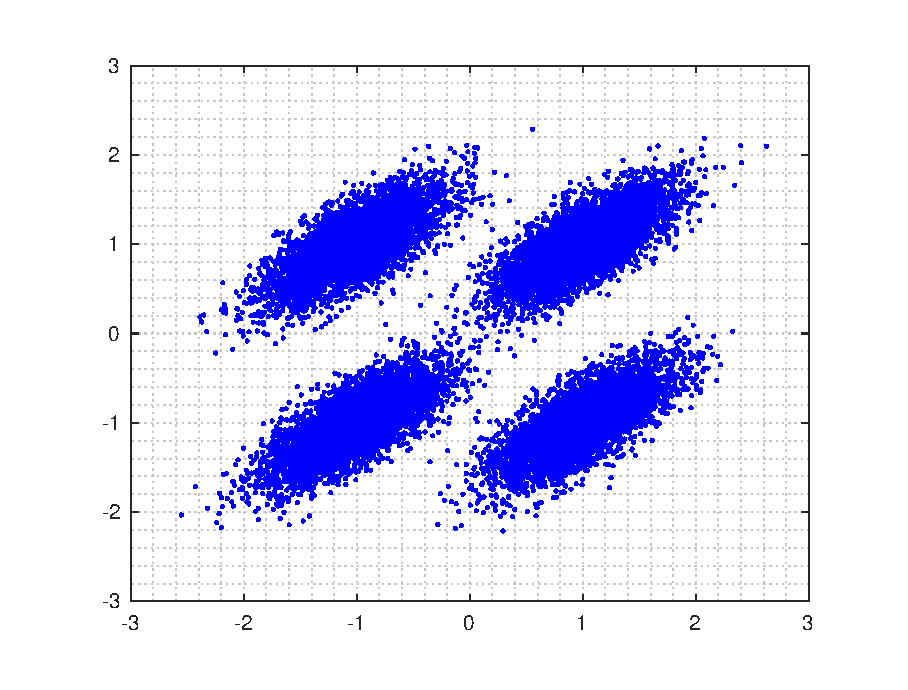
\includegraphics[width=0.49\linewidth]{figuras/rxsymbols}}	
	\subfigure[Constelación de referencia]{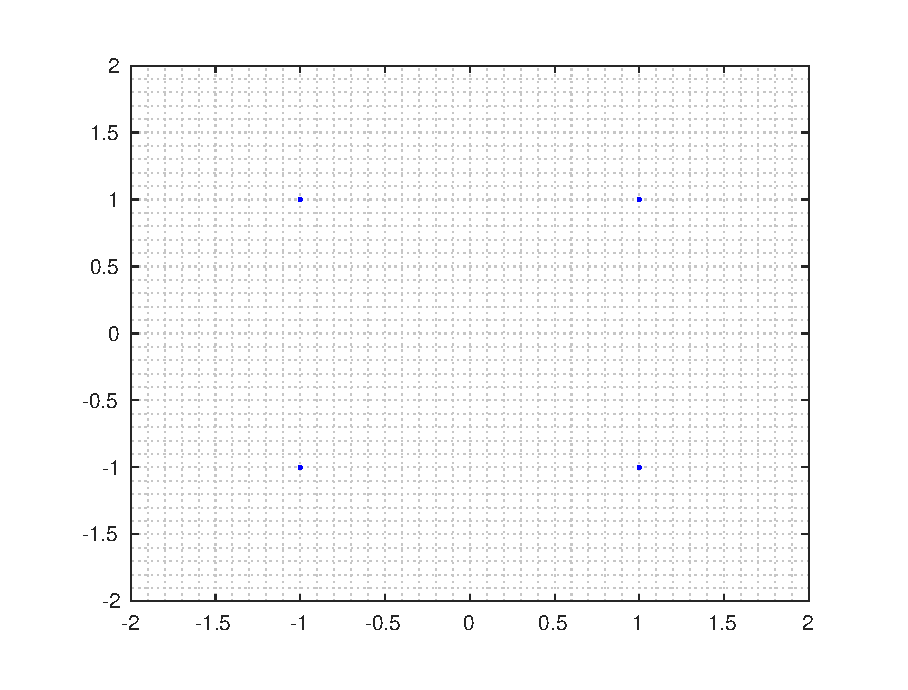
\includegraphics[width=0.49\linewidth]{figuras/rxaConst}}
	\caption{ \textit{Constelaciones a detectar} }
	\label{}
\end{figure}


\subsection{Receptor B}
El receptor B ecualiza los símbolos recibidos multiplicando a los mismos por la matriz inversa de U igual a: $U\cdot \sqrt{D}$, que se la obtiene al multiplicar la matrices $U$ y $D$ producidas por descomposición en valores singulares de la matriz de covarianza $C_G$.
\begin{equation}
	S_{EQ} = U^{-1} \cdot S_{RX} = U^{-1} \cdot (S_{TX} + U \cdot Z) = U^{-1} \cdot S_{TX} + Z
\end{equation}
Esto último elimina la correlación del ruido (convirtiéndolo en ruido gaussiano normalizado) pero modifica la posición de los símbolos de referencia según la transformación $S_{TX}^{(U)} = U^{-1}S_{TX}$. El proceso de detección consiste, al igual que el receptor A, en determinar cual es el símbolo $S_{TX}^{(U)}$ con menor distancia Euclidiana al símbolo $S_{EQ}$.
\begin{figure}[H]
	\centering
	\subfigure[Constelación Ecualizada $S_{EQ}$]{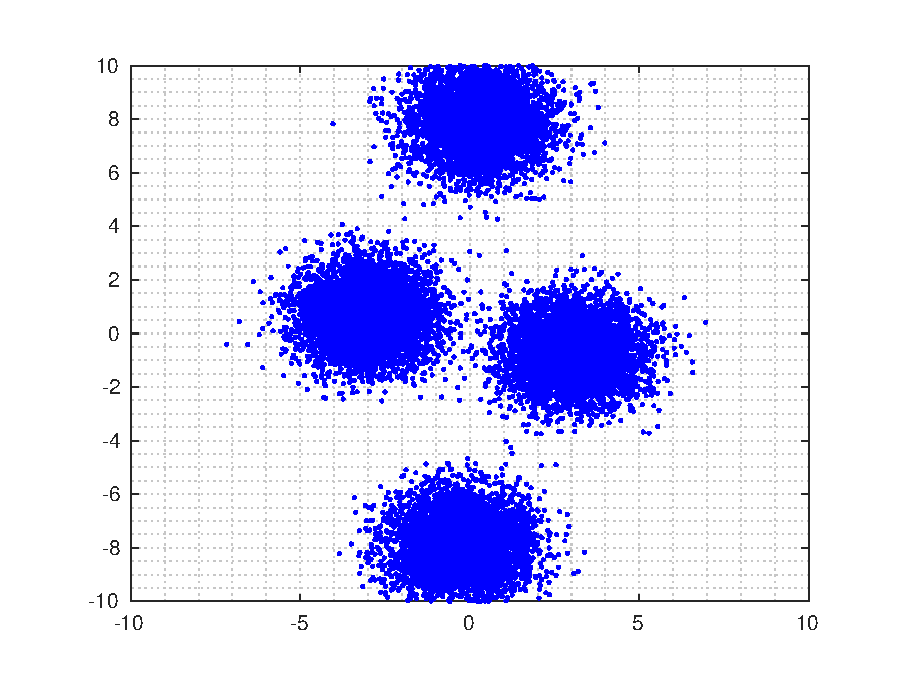
\includegraphics[width=0.49\linewidth]{figuras/rxbEqua}}	
	\subfigure[Constelación de referencia $S_{TX}^{(U)}$]{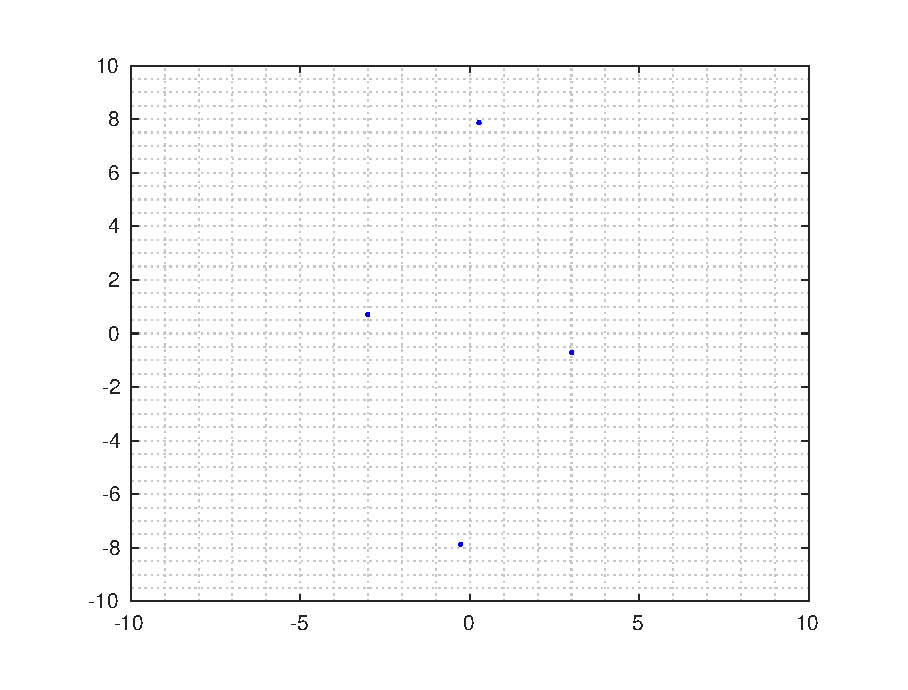
\includegraphics[width=0.49\linewidth]{figuras/rxbConst}}
	\caption{ \textit{Constelaciones a detectar} }
	\label{}
\end{figure}

El siguiente código en Matlab describe el proceso de ecualización y detección mencionado anteriormente. Una vez detectado los símbolos ecualizados, es necesario multiplicarlos de nuevo por la Matriz $U$ para volver a llevarlos a su posición original y de esta manera lograr calcular el error con respecto  a los símbolos generados originalmente \textit{tx\_symbols}.
\begin{minted}[fontsize=\small]{Matlab}
% Receiver B
RxB_Const         = (inv(U)*(RxA_Const'))';
RxB_eq_rx_symbols = inv(U)*rx_symbols;
RxB_eq_dt_symbols = detector(RxB_eq_rx_symbols, RxB_Const);
RxB_dt_symbols    = U * RxB_eq_dt_symbols;
RxB_er_symbols    = sum(sum(abs(RxB_dt_symbols - tx_symbols)) > 1e-10);
RxB_SER(SNR_dB)   = RxB_er_symbols/M
\end{minted}


\subsection{Receptor C}
El receptor C elige el símbolo transmitido que posea mayor probabilidad de haber sido transmitido dado el símbolo recibido. Para realizar este cálculo es necesario utilizar la PDF conjunta de G (ruido gaussiano que ha sido modificado por la matriz $U$).
La función de distribución de probabilidad esta definida como:
\[ 	f_{\bar{X}}(\bar{x})=
	(2\pi)^{-n/2} [\textit{det}(C)]^{-1/2} \textit{exp} \left[ -\dfrac{1}{2} (\bar{x}-\mu)^H C^{-1} (\bar{x}-\mu) \right] \]

Por medio de Matlab se realiza un a función de detección optima que evalúa solo el exponente de la función $f_{\bar{X}}(\bar{x})$, en este caso $\bar{X}$ representará el el vector aleatorio de ruido $G$, y $C$ la matriz de covarianza del ruido.
\begin{minted}[fontsize=\small]{Matlab}
% Calculo de la PDF
x         = rx_symbols(:,k) - const(n,:)';
dists2(n) = x' * invC * x;
\end{minted}

La señal recibida por el receptor C es igual a la recibida por el receptor A que luego es comparado con los símbolos de referencia [1 1; 1 -1; -1 1; -1 -1], la única diferencia consiste en la forma de detección. Evaluando los tres receptores en una única gráfica: 
\begin{figure}[H]
	\centering
	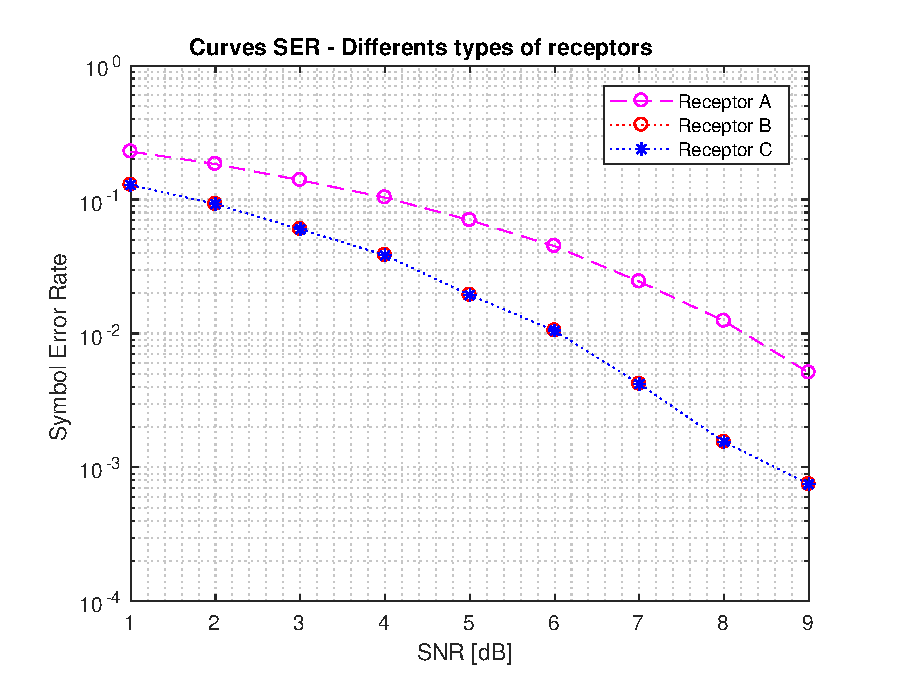
\includegraphics[width=0.7\linewidth]{figuras/Curves}
	\caption{\textit{Symbol Error Rate de los tres receptores}}
	\label{fig:curves}
\end{figure}


\newpage
\section*{Anexo}
$\bullet$ Una descomposición en valores singulares de una matriz A es una factorización $A=U\Sigma V^T$, donde $U$ es matriz unitaria $(U.U^T=I)$, $\Sigma$ es matriz diagonal y $V$ es matriz unitaria, a $U$ y $V$ también se las llama matrices ortogonales. Una Matriz Ortogonal es aquella matriz que multiplicada por su traspuesta da como resultado la matriz identidad o unidad: $M.M^T=I$.
\\
$\bullet$ Interpretación geométrica de los valores singulares: consideremos una esfera unitaria $S$ en $R^2$, la transformación ortogonal $V$ sólo produce la rotación de la esfera S, $\Sigma$ la deforma en una hiperelipse y finalmente $U$ rota la hiperelipse.
\\
$\bullet$ La matriz de covarianza C asociada a un vector $\bar{X}$.
\begin{equation}
C_{\bar{X}} = 
\begin{bmatrix}
	\sigma_{X_1}^2 		& \sigma_{X_1,X_2}^2 \\
	\sigma_{X_2,X_1}^2 	& \sigma_{X_2}^2
\end{bmatrix}
\end{equation}
\\
$\bullet$ Sea $\bar{X} \sim \mathcal{N}(\mu,\textbf{C})$, donde $\bar{X}=\left[ X_1,X_2,\dots,X_n \right]^T$ es un vector aleatorio de media $\mu$ y covarianza $\textbf{C}$. Con función de distribución de densidad:
\begin{equation}
	f_{\bar{X}}(\bar{x})=
	(2\pi)^{-n/2} [\textit{det}(C)]^{-1/2} \textit{exp} \left[ -\dfrac{1}{2} (\bar{x}-\mu)^H C^{-1} (\bar{x}-\mu) \right] 
\end{equation}
\\
$\bullet$ La distancia euclidiana entre los puntos ${P=(p_{1},p_{2},\dots ,p_{n})}$ y ${Q=(q_{1},q_{2},\dots ,q_{n})\,}$, del espacio euclídeo n-dimensional, se define como:
\begin{equation}
d_{E}(P,Q)={\sqrt {\sum _{i=1}^{n}(p_{i}-q_{i})^{2}}}
\end{equation}
\\
Una vista matemática para calcular la mínima distancia en el receptor A: 
\[ \sum(rxA - SymbComp')^2 \]
Para el caso del receptor C, se emplea sólo el exponente de la función de distribución de probabilidad: 
\[ (rxC - SymbComp')' \cdot inv(C_G) \cdot (rxC - SymbComp') \]



\end{document}
